\subsubsection{2.2. Mô hình embedding câu (Sentence Transformer)}
\indent\indent Trong các bài toán xử lý ngôn ngữ tự nhiên (NLP) hiện đại, việc chuyển đổi văn bản thành các vector số thực (embeddings) là bước tiên quyết để máy tính có thể hiểu và xử lý ngữ nghĩa. Khác với các phương pháp truyền thống như Bag-of-Words hay TF-IDF dựa trên tần suất từ, các mô hình embedding hiện đại ánh xạ văn bản vào một không gian vector, nơi các câu có ngữ nghĩa tương đồng sẽ nằm gần nhau về mặt hình học.\vspace{0.3cm}

Mặc dù các mô hình ngôn ngữ lớn như BERT (Bidirectional Encoder Representations from Transformers) đạt hiệu quả cao trong nhiều tác vụ, chúng lại không tối ưu cho việc tạo ra vector biểu diễn ở cấp độ câu (sentence embeddings). Để giải quyết vấn đề này, Reimers và Gurevych \cite{reimers2019sentencebertsentenceembeddingsusing} đã giới thiệu Sentence-BERT (SBERT), một sửa đổi của kiến trúc BERT sử dụng Siamese networks để trích xuất các đặc trưng ngữ nghĩa.\vspace{0.3cm}

\begin{figure}[H]
    \centering
    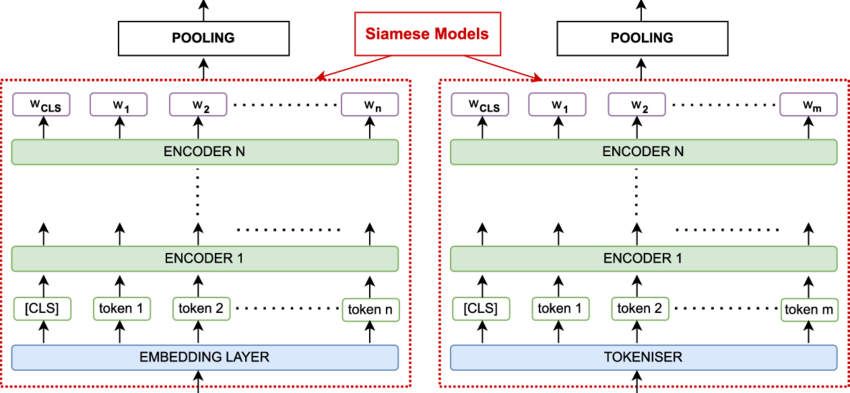
\includegraphics[width=0.8\linewidth]{images/part-02/chap-01/SBERT.png}
    \vspace{0.5cm}
    \caption{Minh hoạ kiến trúc cơ bản của SBERT}
    \label{fig:SBERT}
\end{figure}

Cơ chế hoạt động của SBERT như sau:\vspace{-0.1cm}
\begin{itemize}[label={--}, itemsep=1pt]
    \item Siamese Architecture: Hai câu văn bản đầu vào được đưa qua cùng một mạng BERT (chia sẻ trọng số) để tạo ra các vector ngữ cảnh.
    \item Pooling Strategy: Một lớp Pooling (thường là Mean Pooling) được áp dụng để nén thông tin từ các token thành một vector cố định đại diện cho toàn bộ câu.
    \item Objective Function: Trong quá trình huấn luyện, mạng tối ưu hóa hàm mất mát (như Cosine Similarity Loss) để kéo các vector của các câu có nghĩa giống nhau lại gần và đẩy các câu khác nghĩa ra xa.
\end{itemize}

Trong thực tế triển khai, các mô hình BERT chuẩn (như BERT-base) là rất nặng và chậm. Để cân bằng giữa hiệu suất và tốc độ, Wang và cộng sự đã thiết kế kiến trúc MiniLM \cite{wang2020minilmdeepselfattentiondistillation} dựa trên kỹ thuật chưng cất tri thức (Knowledge Distillation).\vspace{0.3cm}

Mô hình all-MiniLM-L6-v2 là một trong những đại diện phổ biến nhất của dòng này (được triển khai trong thư viện \textit{sentence-transformers}), với các đặc điểm kỹ thuật sau:\vspace{-0.1cm}
\begin{itemize}[label={--}, itemsep=1pt]
    \item Kiến trúc: Sử dụng MiniLM làm nền tảng, mô hình này đóng vai trò là "học sinh" (student) học lại tri thức từ các mô hình "giáo viên" (teacher) lớn hơn như BERT hoặc RoBERTa. Đặc biệt, MiniLM chưng cất cả mối quan hệ self-attention thay vì chỉ chưng cất lớp đầu ra, giúp mô hình nhỏ giữ được khả năng hiểu ngữ cảnh sâu.
    \item Cấu hình: Ký hiệu "L6" biểu thị mô hình chỉ có 6 lớp Transformer (so với 12 lớp của BERT-base), giúp giảm kích thước mô hình xuống khoảng 80MB và tăng tốc độ suy luận lên hơn 5 lần.
    \item Biểu diễn: Đầu ra là một vector có kích thước 384 chiều. Mặc dù số chiều nhỏ hơn so với chuẩn 768 của BERT, all-MiniLM-L6-v2 vẫn duy trì độ chính xác cao trên các bảng xếp hạng đánh giá embedding (như MTEB), đặc biệt hiệu quả cho các tác vụ tìm kiếm ngữ nghĩa và gom nhóm văn bản.
\end{itemize}